\begin{flushright} {\tiny {\color{gray} adiabatic.tex}} \end{flushright}
%~~~~~~~~~~~~~~~~~~~~~~~~~~~~~~~~~~~~~~~~~~~~~~~~~~~~~~~~~~~~~~~~~~~~~~~~~~~~~~~~~~~~~~~~~~~~~~~~~~

We start by the first sentence of Bunge (2005) \cite{bung05}:
"The average temperature increase through Earth's
crust and mantle is called the geotherm. Its basic form is
assumed to consist of adiabatic regions where temperatures 
rise only slightly with depth, and of narrow thermal
boundary layers where temperatures increase rapidly
over a depth of a few hundred kilometers (Jeanloz and
Morris, 1986) \cite{jemo86}."

Before we look further at the equations behind this temperature profile, 
we must look at the basic assumption we make about
the type of convection taking place in the mantle:
layered convection vs. whole mantle convection, as
depicted here: 

\begin{center}
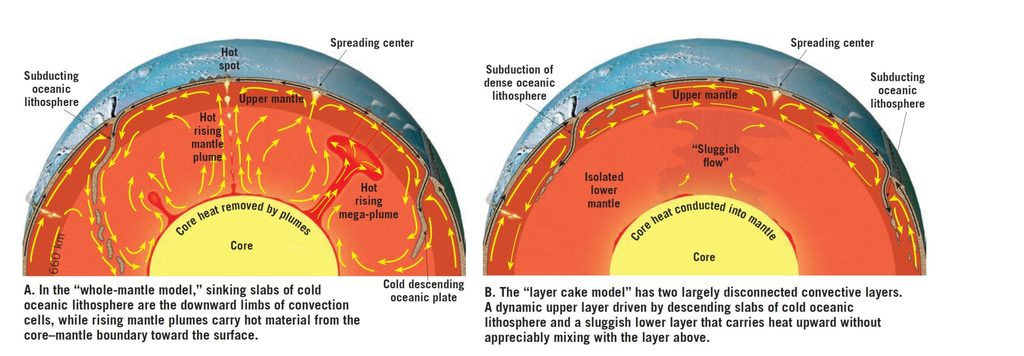
\includegraphics[width=12cm]{images/adiabatic/modes}\\
{\captionfont Taken from \url{https://geologyengineering.com/2020/05/mantle-convection/}}
\end{center}

\noindent Indeed, the type of convection is then expected to have an strong influence 
on the radial temperature profile: 

\begin{center}
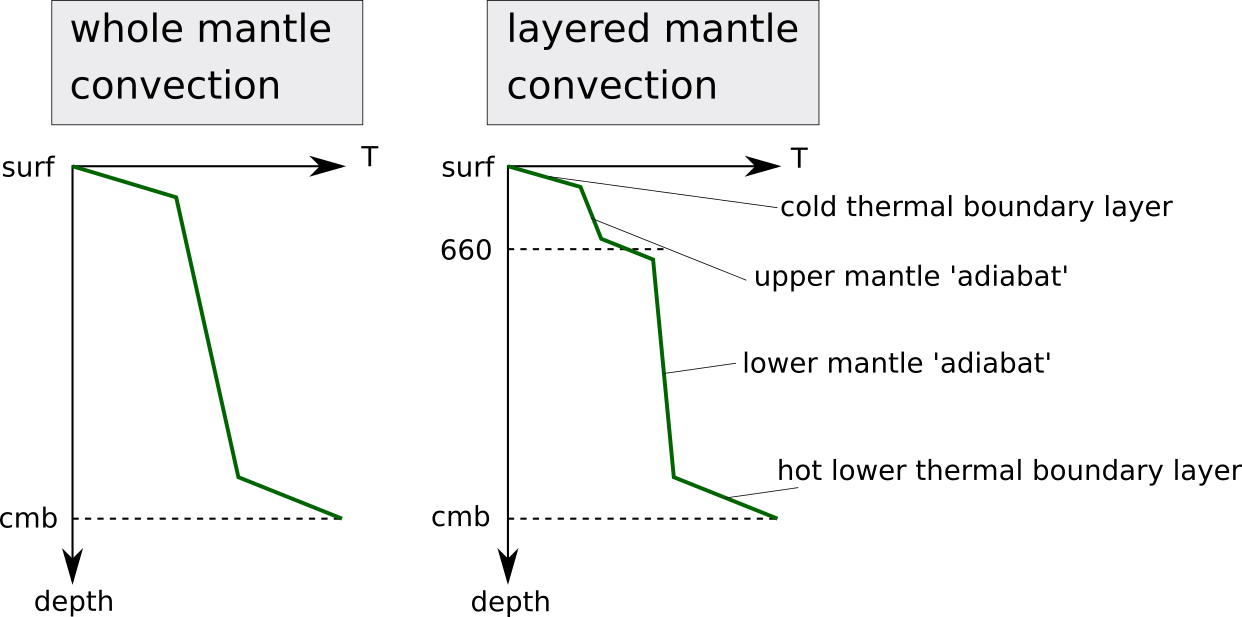
\includegraphics[width=10cm]{images/adiabatic/drawing.png}
\end{center}

This is also to be found in Poirier's book \cite{poirier}:
\begin{center}
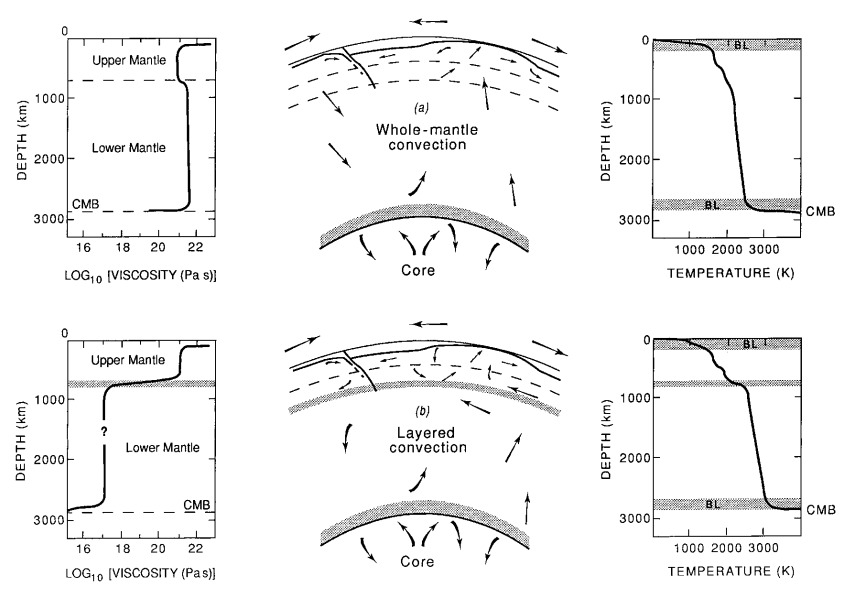
\includegraphics[width=11cm]{images/adiabatic/poirier}\\
{\captionfont Schematic diagrams of (a) whole-mantle and (b) layered convection
models, with corresponding temperature and viscosity profiles (after 
Peltier \& Jarvis (1982) \cite{peja82}.)}
\end{center}


The two-layered convection hypothesis relies essentially 
on the viscosity jump at the 660 discontinuity and seems 
to be generally accepted.
It also forms the basis of {\v{C}}adek \& van den Berg (1998) \cite{cava98}
in which the authors carry out an inversion to obtain 
radial profiles of temperature and viscosity in the Earth's mantle
inferred from the geoid and lateral seismic structure:
\begin{center}
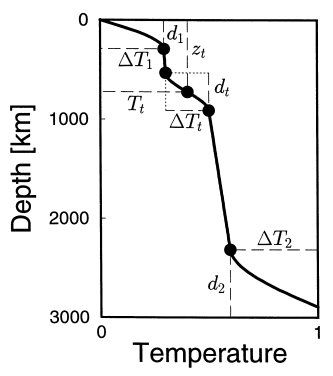
\includegraphics[width=6cm]{images/adiabatic/cava98a.png}
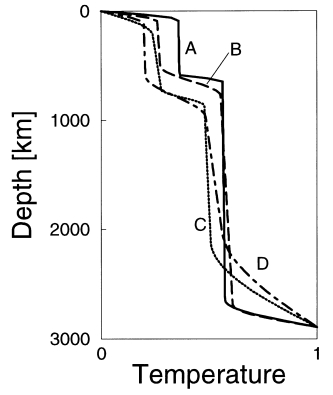
\includegraphics[width=5.5cm]{images/adiabatic/cava98b.png}\\
{\captionfont Taken from \cite{cava98}. 
Left: Parameterization of the geotherm used in the paper;
Right: Four model geotherms reducing the misfit by 70\%. The
differences between the models illustrate uncertainties of the
solution.}
\end{center}

More recently, Katsura \etal (2010) \cite{kayy10} have constructed the following mantle temperature 
and temperature gradient profiles:

\begin{center}
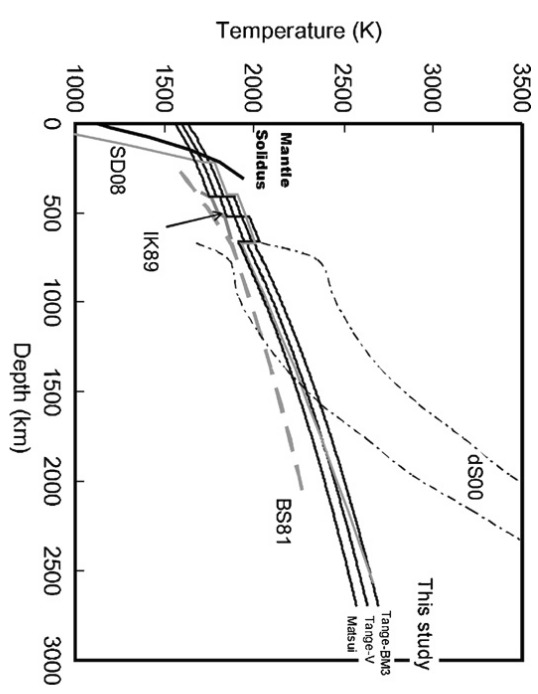
\includegraphics[width=6cm]{images/adiabatic/kayy10a}
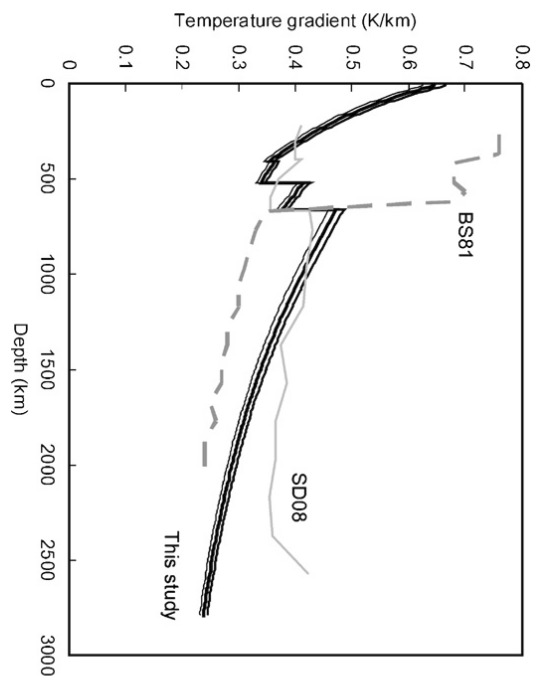
\includegraphics[width=6cm]{images/adiabatic/kayy10b}\\
{\captionfont Taken from Katsura \etal (2010) \cite{kayy10}.
Left: The adiabatic temperature distributions in the mantle. The three solid lines
denote the temperature distributions proposed in this study using three different
pressure scales. Those proposed by the previous studies are shown for comparison
(BS81: Brown and Shankland, 1981; IK89: Ito and Katsura, 1989; dS00: da Silva \etal,
2000; SD08: Stacey and Davis, 2008). The mantle solidus proposed by Hirschmann
(2000) is also shown.
Right:
Adiabatic temperature gradient in the mantle. The adiabatic temperature gradient 
abruptly increases in association with the olivine-wadsleyite,
wadsleyite-ringwoodite, ringwoodite-perovskite + periclase transitions, as is the
case for the thermal expansion. The adiabatic temperature gradients given in the
previous studies are also shown for comparison (BS81: Brown and Shankland, 1981;
SD08: Stacey and Davis, 2008 \cite{stacey_davis}).
}
\end{center}


\begin{center}
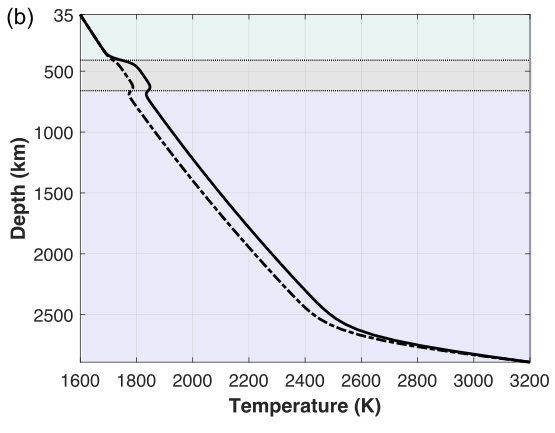
\includegraphics[width=10cm]{images/adiabatic/nemi23}\\
{\captionfont Taken from \textcite{nemi23}.}
\end{center}


Prof. Steinberger was gracious to communicate to me the data of Steinberger \& Calderwood (2006) \cite{stca06}:
\begin{center}
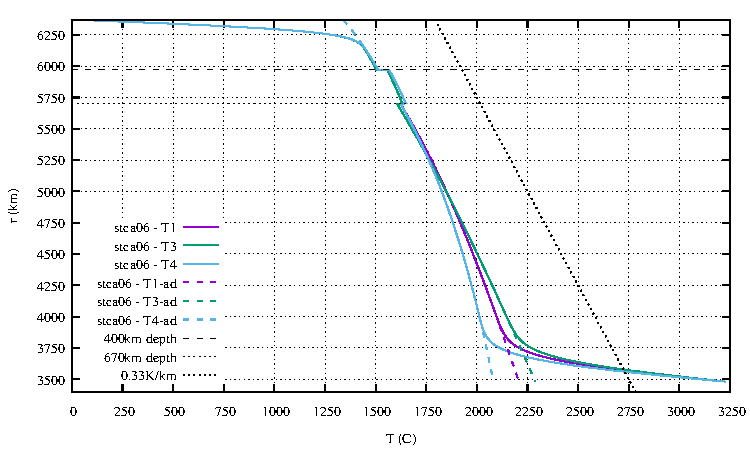
\includegraphics[width=8.5cm]{images/adiabatic/steinberger/Tprofile.pdf}
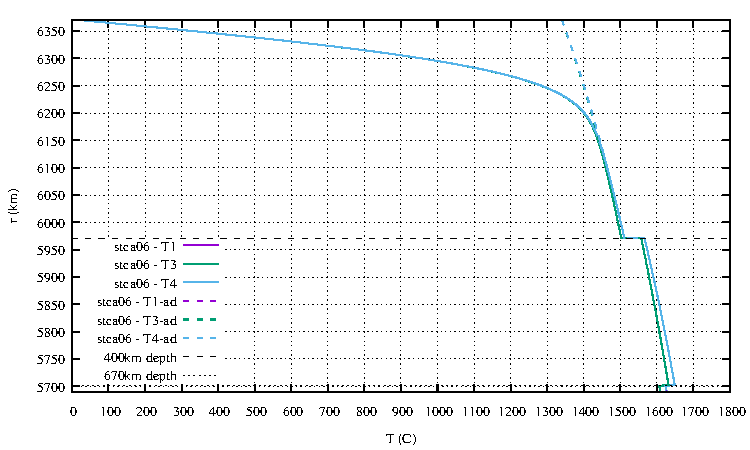
\includegraphics[width=8.5cm]{images/adiabatic/steinberger/Tprofile_upper.pdf}\\
{\captionfont Temperature profiles from Steinberger \& Calderwood \cite{stca06}.}
\end{center}

One can gather data from various papers and books and this yields the following 
figure\footnote{It must be said that finding actual data -not figures- is remarkably difficult.}:

\begin{center}
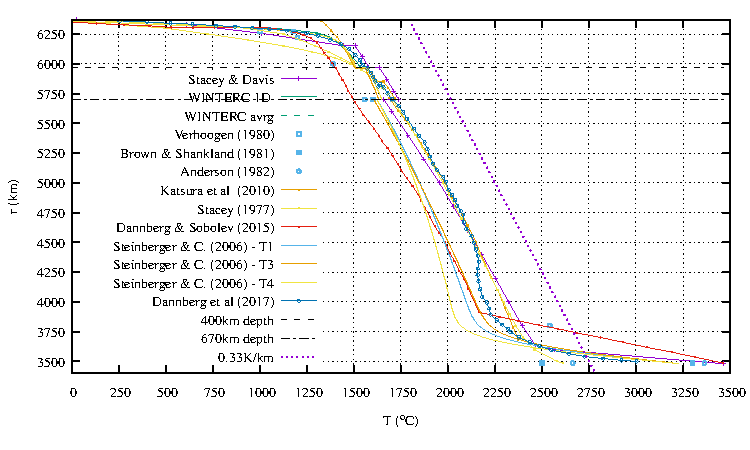
\includegraphics[width=8.5cm]{images/adiabatic/Tprofile.pdf}
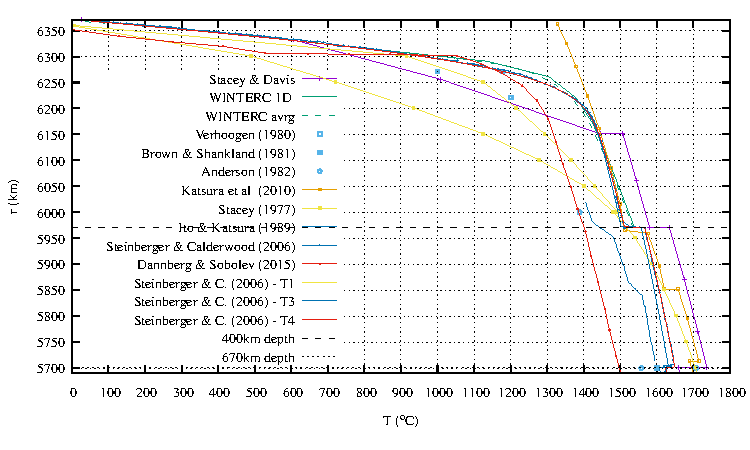
\includegraphics[width=8.5cm]{images/adiabatic/Tprofile_upper.pdf}\\
{\captionfont 
Note that the T values of Stacey (1977) \cite{stac77} inexplicably go to 540-550K at the surface. 
The value 545 has therefore been subtracted from the values in the paper. These then 
align remarquably well with those of Katsura \etal
}
\end{center}




We see that there is a remarkable agreement between many studies for the temperature down to 400km 
depth. Most show a step in the profile between 400 and 670km depth but the temperature at 670km
depth seems to be between 1650$\si{\celsius}$ and 1750$\si{\celsius}$.
Further down, the discrepancy between studies increases (effectively boiling down to 
the value of the adiabatic gradient). 100km above the CMB all studies seem to indicate a 
temperature of 2300-2400$\si{\celsius}$. Temperature values at the CMB differ a lot and 
as noted in Bull \etal (2009) \cite{bumr09}: 
"Estimates of CMB temperature vary greatly. [...] 
We impose a surface temperature of 273 K and
investigate three CMB temperatures: 3000 K (consistent with
previous studies of this nature, e.g., Kellogg \etal., 1999 \cite{kehv99}), 3950 K
(consistent with recent results on the double-crossing of Post-
Perovskite, e.g., Hernlund \etal., 2005 \cite{hett05}; van der Hilst \etal, 
2007 \cite{vadw07}; Alf\`e \etal., 2002), and 4800 K (Knittle and Jeanloz, 1991). The 3950 K
temperature is the 'reference' temperature which we use for the
majority of cases."
The CMB temperature is set to $2900-3200\si{\celsius}$ in Fowler \cite{fowler}.


Also, oceanic plates being thinner than continental plates (alongside with different 
radiogenic decay and thermal properties) one can draw two representative mantle 
geotherms \cite{tusc}:

\begin{center}
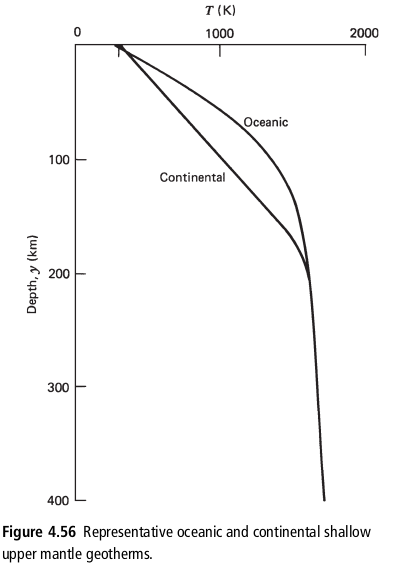
\includegraphics[width=4cm]{images/adiabatic/tusc.png}\\
{\captionfont Taken from Turcotte \& Schubert \cite{tusc}}
\end{center}



\begin{center}
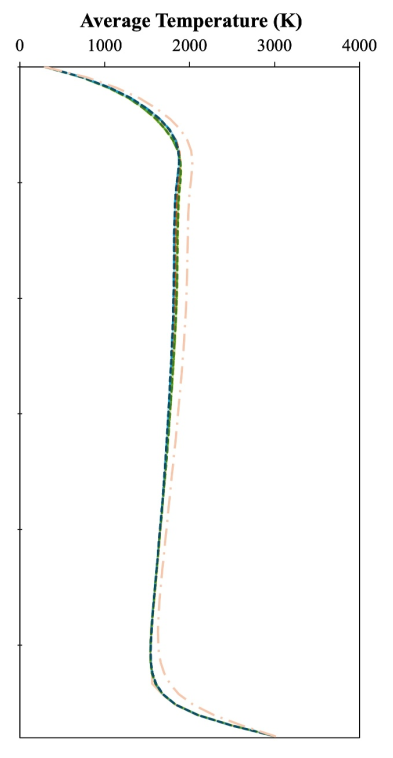
\includegraphics[width=6cm]{images/adiabatic/pldp24}\\
{\captionfont \twothousandtwentyfour: Taken from \textcite{pldp24} (2024).}
\end{center}

\newpage


The following paragraph is from B. Steinberger oct 26th, 2020
(personnal communication):

\begin{displayquote}
I think the temperature below the lithosphere is still fairly well-constrained, 
based on magmas produced on mid-oceanic ridges (away from plumes) if one takes 
these as representative. Regarding Dannberg and Sobolev (not Solomatov!) 
I don't know why it is lower. In their supplementary figures, the extrapolation 
to the surface is actually $\sim 1250\si{\kelvin}$, not $1250\si{\celsius}$, 
which is even less. Perhaps best to directly ask Juliane about this.

How the temperature increases with depth is more uncertain; the temperature 
gradient is often taken as adiabatic; that's what I also assumed in the 2006 
paper, then it is defined by a ordinary differential equation (eq. 12 in that paper). 
I think the main uncertainty is the thermal expansivity. In my model, it strongly 
decreases with depth, I guess that is why my models have a lower temperature in 
the lower mantle than other models. I think that strong decrease in expansivity 
is still the consensus, but I didn't closely follow the literature recently. 
But the temperature gradient between the thermal boundary layers may actually 
be subadiabatic, hence even lower, due to cold slabs sinking to and accumulating 
above the CMB, and hot plume material feeding into the asthenosphere, below the 
lithosphere. So, yes, I would say the difference in the deep mantle (if not more) 
reflects the current state in the community.
I think the uncertainites of CMB temperature are even larger. 
\end{displayquote}



\Literature: 
\begin{itemize}
\item \fullcite{jape82}
\item \fullcite{king15}
\item \fullcite{tiro16}
\end{itemize}


check section 7.7 in Fowler !


